\chapter{Deep Learning}
Deep learning has recently been highly successful in machine learning across a variety of application domains, including computer vision, natural language processing, and big data analysis, among others. For example, deep learning methods have consistently outperformed traditional methods for object recognition and detection in the ISLVRC Computer Vision Competition since 2012 \cite{ILSVRC15}. However, deep learning’s high accuracy comes at the expense of high computational and memory requirements for both the training and inference phases of deep learning. Training a deep learning model is space and computationally expensive due to millions of parameters that need to be iteratively refined over multiple time epochs. Inference is computationally expensive due to the potentially high dimensionality of the input data (e.g., a high-resolution image) and millions of computations that need to be performed on the input data.

\section{Background}
As described in \cite{Goodfellow-et-al-2016}, the modern term “deep learning” goes beyond the neuroscientific perspective engineering applications on the current breed of machine learning models. It appeals to a more general principle of learning \textit{multiple levels of composition}, which can be applied in machine learning frameworks that are not necessarily neurally inspired.
A deep learning prediction algorithm, consists of a number of layers, as shown in Fig. \ref{fig:dnn}.

\begin{figure}
	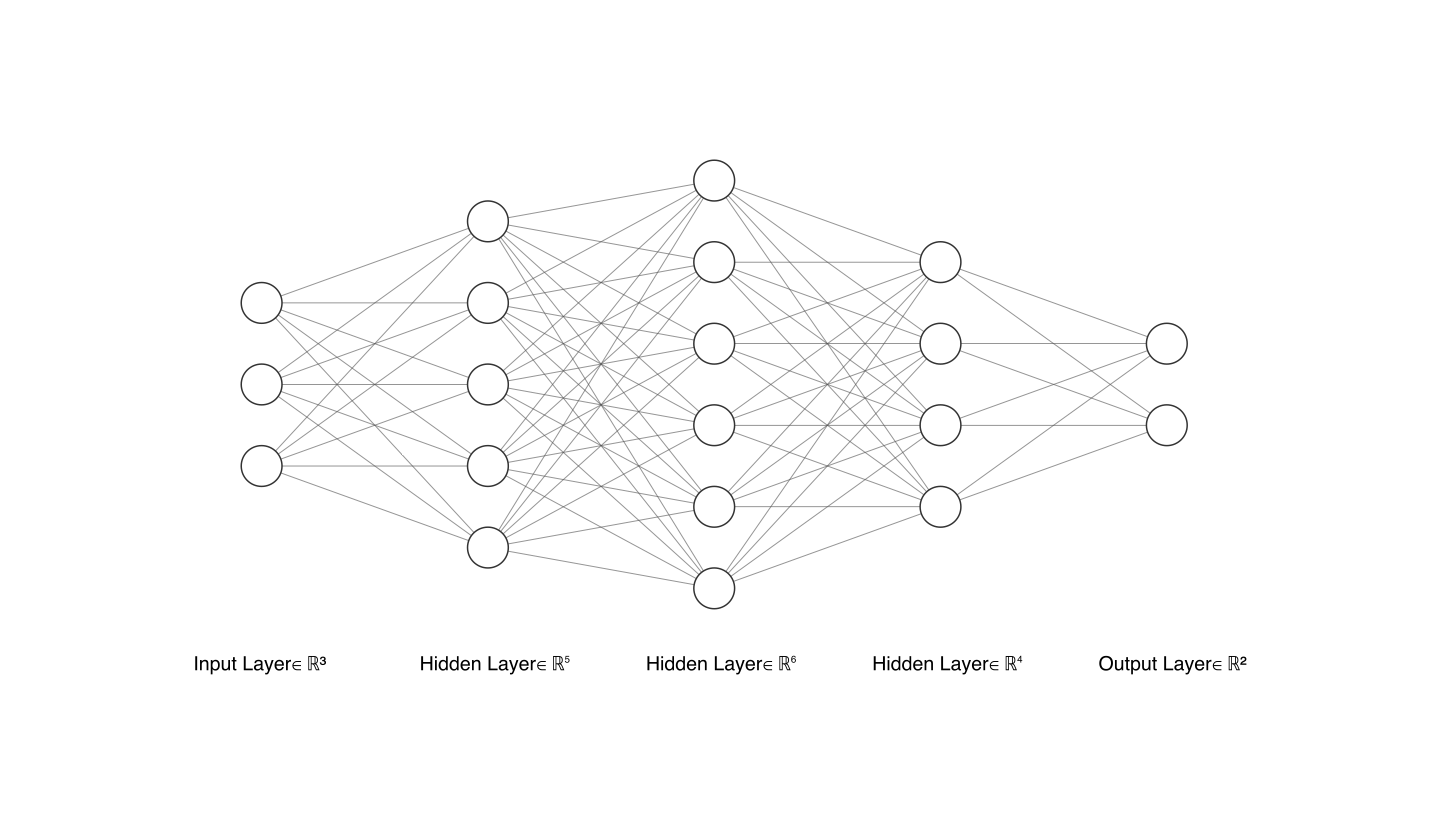
\includegraphics[width=\textwidth]{images/nn.png}
	\caption[DNN example]{DNN example with image classification}
	\label{fig:dnn}
\end{figure}

In deep learning \textit{inference}, the input data pass through the node's layers in sequence, and each layer performs matrix multiplications on the data. The output of a layer is usually the input to the subsequent layer. After data are processed by the final (fully connected) layer, the output is either a feature or a classification value. When the model contains many layers in sequence, the neural network is known as a deep neural network (DNN). When the matrix multiplications include convolutional filter operations, the model is named convolutional neural networks (CNNs), which is common for image and video processing contexts. There are also DNNs designed especially for time series prediction; these are called recurrent neural networks (RNNs), which have loops in their layer connections to keep state and enable predictions on sequential inputs.

In deep learning \textit{training}, the computation proceeds in reverse order. Given the ground-truth training labels, multiple passes are made over the layers to optimize the parameters of each layer of matrix multiplications, starting from the final layer and ending with the first layer. The algorithm used is typically stochastic gradient descent (SGD).  In each pass, a randomly small subset of N input data ("mini-batch") from the training data set, is selected and used to update the gradients in the direction that minimizes the training loss (where the training loss is defined as the difference between the predictions and the ground truth). One pass through the entire training data set is called a training epoch \cite{ruder2016overview}.

There are some considerations to take into account: the first is that there are a large number of parameters in the matrix multiplications, resulting in many computations being performed and thus the latency issues that we see on end devices. The second is that there are many choices (hyper-parameters) on how to design the DNN models (e.g., the number of parameters per layer, and the number of layers), which makes the model design more of an art than a science. Different DNN design decisions result in tradeoffs between system metrics; for example, a DNN with higher accuracy likely requires more memory to store all the model parameters and will have higher latency because of all the matrix multiplications being performed. On the other hand, a DNN model with fewer parameters will likely execute more quickly and use less computational resources and energy, but it may not have sufficient accuracy to meet the application's requirements.


\section{Measurement}
How can we evaluate the performance of a neural network?



\section{Frameworks}


\section{Challenges}

\section{Discussion}
Needle insertion is a complex procedure that involves a non-trivial effect, needle's bending, which is also non-trivial both to model an control.
When performing this action the clinician relays on kinestetic feedback and visual feedback. The former provides information on the moment of punturing and the tissiue tipe, the latter gives a feedback on the target and also on tissues type.
The needle bending could be exploited expecially by robotic procedures to provide a more precise target reaching and to avoid ostacle on the insertion path.

In order to design a fully automated system a precise model of the forces acting on the needle, a clear identification of punturing stages (pre, post andpuncturing) and a predictive model of tissue deformation are needed to develop control strategies and path plannig. The system also need a feedback that should provide needle and target tracking, and information on the environment like the interaction forces.
Engineering and integrating such a system is really challenging.
Becouse of the surgeon expertise with challenging task and unexpected situations the preffered clinical solution is to develop a robotic assited device that assists the operator in the positioning phase but demands to the clinician the insertion phase.

Telerobotics could be a valuable solution to put clinitian's expertise in the loop while enhancing the procedure's precision. However it has to deal with the classical teleoperation trade off between stability and transparency as we will discuss in the following chapter. In particular for the punturing action the main issue is the abrupt change in the force at the puncturing time which may induce in the operator an unwanted refletion feedback that breaks the transparency. 
%%%%%%%%%%%%%%%%%%%%%%%%%%%%%%%%%%%%


\clearpage
\thispagestyle{empty}